
\section{Introduction}
Considering the generation process described by LDA, it is notable
that, the documents are independent given the LDA model.  This
property makes it possible to design a distributed Gibbs sampling
algorithm for learning LDA \cite{dist-lda-gibbs}.  Also, this makes it
possible to develop this algorithm using MapReduce.


\section{Scalable Training}
\label{sec:model_train}

\begin{figure}
  \centering
  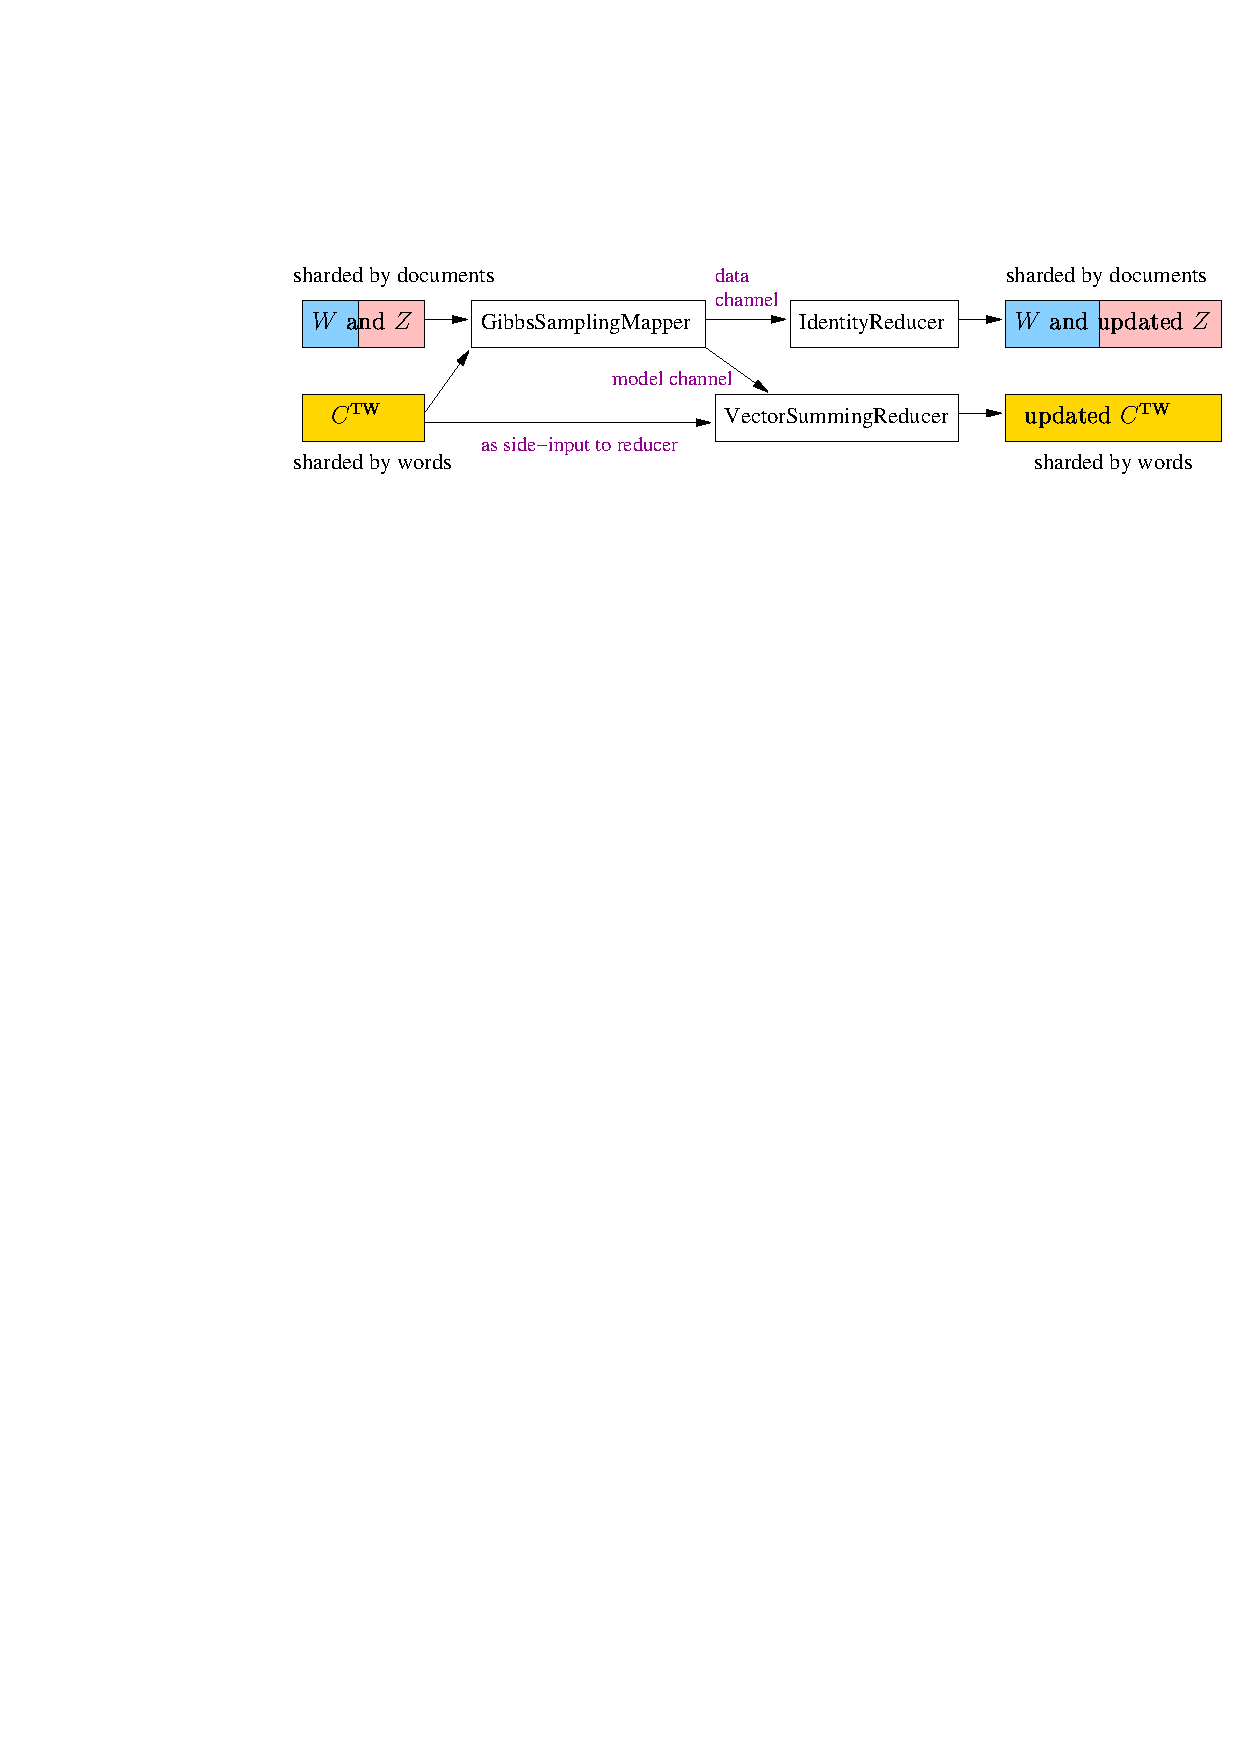
\includegraphics[width=\columnwidth]{lda-mapreduce}
  \caption{The framework of MapReduce-LDA}
  \label{fig:mapreduce-lda}
\end{figure}

In order to support large-scale image annotation, we adopt a
distributed Gibbs sampling algorithm, AD-LDA, proposed in
\cite{dist-lda-gibbs}.  The basic idea is to divide the training
corpus into $P$ parts, each part is saved on one computer.  Each
computer executes one iteration of the Gibbs sampling
algorithm~\cite{lda_gibbs} to update its local model using its local
data, and then the $P$ local models are summed up to form the global
model, which is replicated to the $P$ computers to support the next
iteration.

Usually, the AD-LDA algorithm can be developed using the MPI
programming model, which is flexible and highly efficient, but does
not support auto fault recovery --- as long as one computer fails
during computation, all computers have to restart their tasks.  This
is not a problem when we use tens of computers.  But to support real
large-scale data like Web images, we need magnitudes more computers.
During the hours long training process, the probability that none of
them fails is close to 0.  Without auto fault recovery, the training
will restart again and again, and statistically, never ends.

We solve this problem by modeling the AD-LDA algorithm by the
MapReduce programming model\cite{mapreduce}, which has been supporting
most Web-scale computations in Google$^\copyright$.  MapReduce takes
input from a set of tuples and outputs tuples.  A set of tuples is
usually distributed stored as subsets known as a ``shards''.  A
MapReduce computation job consists of three stages --- mapping,
shuffling and reducing.  The mapping and shuffling stages are
programmable.  To program the mapping stage, users provide three
functions \texttt{Start()}, \texttt{Map()} and \texttt{Flush}.  For
every shard, a thread known as ``map worker'' is created to invoke
\texttt{Start} once, and then \texttt{Map()} multiple times for each
tuple in the shard, and then \texttt{Reduce()} once.  These functions
can output one or more key-value pairs, which are collected and
aggregated by the shuffling stage.  Key-value pairs that come from
various map workers but share the same key are aggregated into a set
known as a ``reduce input'', and this common key is assigned the key
of the reduce input.  Each reduce input will be processed by an
invocation of the \texttt{Reduce} function, which is provided by the
user.

We model each iteration of AD-LDA by the following MapReduce job:
\begin{description}
\item[\texttt{Start()}] loads the model updated by the previous iteration;
\item[\texttt{Map()}] updates topic assignments of words in a document
  using the model, and records how the model should be updated
  according to the new topic assignments;
\item[\texttt{Flush()}] outputs the recorded update opinion.
\end{description}
Note that both the model as its update opinion are
$V\times{}K$ sparse matrices, where $V$ is the number of unique words
in the training corpus, and $K$ is the number of topics specified by
the user.  \texttt{Flush()} outputs each row of the update opinion
matrix with the key of the corresponding word\footnote{This document is
  based on Google MapReduce implementation.  Another well known
  implementation of the MapReduce model is Hadoop
  (\url{http://hadoop.apache.org}), which does not expose shard
  boundaries to programmers via \texttt{Start()} and
  \texttt{Flush()}.}.  So the shuffling stage aggregates update
opinion rows corresponding to a certain word and coming from various
map workers into a reduce input.  So \texttt{Reduce()} sums the rows
element-wise to get the aggregated update opinion row for a word.  The
update opinion row should be added to the corresponding row of the old
model estimated by the previous iteration.  In a very restrictive
MapReduce model, this has to be done in a separate MapReduce job.
However, most MapReduce implementations now support multiple types of
mappers.  So rows of the old model can be loaded by an IdentityMapper
and sent to \texttt{Reducer()}.
%
It is also notable that we need to save the updated topic assignments
for use in the next iteration.  This can be done in \texttt{Map()},
because each document is processed once in each iteration.

%%%%%%%%%%%%%%%%%%%%%%%%%%%%
\section{Scalable Model Selection}
\label{sec:model_select}
%%%%%%%%%%%%%%%%%%%%%%%%%%%%

We have mentioned two parameters of the above training algorithm: the
vocabulary importance factor $\gamma$ and the number of topics $K$.
Values of these parameters can be determined by cross-validation ---
given any pair of $\langle{\gamma,K}\rangle$, we train a
two-vocabulary LDA using part of data (known as ``training data'') and
then compute the perplexity of the rest data (known as ``testing
data'') given the trained model~\cite{heinrich}.  The smaller the
perplexity value, the better that the model explains the data.  To
support large-scale testing data, we model the computation of
perplexity by MapReduce:
\begin{description}
\item[\texttt{Start()}] loads the model;
\item[\texttt{Map()}] computes the log-likelihood $\LL$ of the current
  document given the model, and outputs a key-value pair, where key is
  a constant value, which makes all outputs being packed into one
  reduce input; value is a pair $\langle{\LL_d,N(d)}\rangle$, where
  $N(d)$ is the length of document $d$;
\item[\texttt{Reduce()}] output perplexity
  ${perp}=\exp\left[\sum_d\LL_d/\sum_d N(d)\right]$.
\end{description}


\section{Experiments Using Synthetic Data}

\begin{figure}[!t]
  \centering
  
\includegraphics[width=2.3cm]{griffith-images/shengxiao/gou}
  
\includegraphics[width=2.3cm]{griffith-images/shengxiao/hou}
  
\includegraphics[width=2.3cm]{griffith-images/shengxiao/hu}
  
\includegraphics[width=2.3cm]{griffith-images/shengxiao/ji}
  
\includegraphics[width=2.3cm]{griffith-images/shengxiao/long}
  
\includegraphics[width=2.3cm]{griffith-images/shengxiao/ma}
  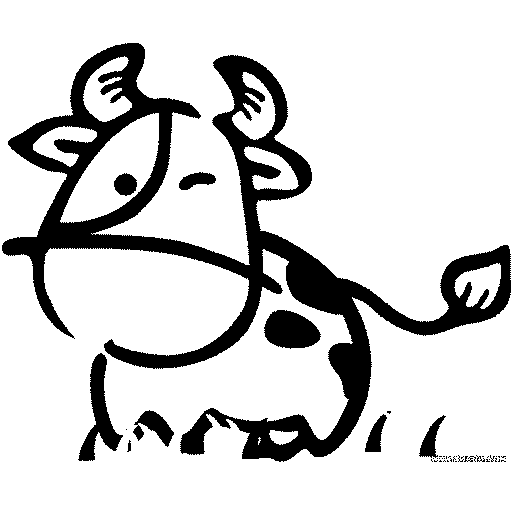
\includegraphics[width=2.3cm]{griffith-images/shengxiao/niu}
  
\includegraphics[width=2.3cm]{griffith-images/shengxiao/she}
  
\includegraphics[width=2.3cm]{griffith-images/shengxiao/shu}
  
\includegraphics[width=2.3cm]{griffith-images/shengxiao/tu}
  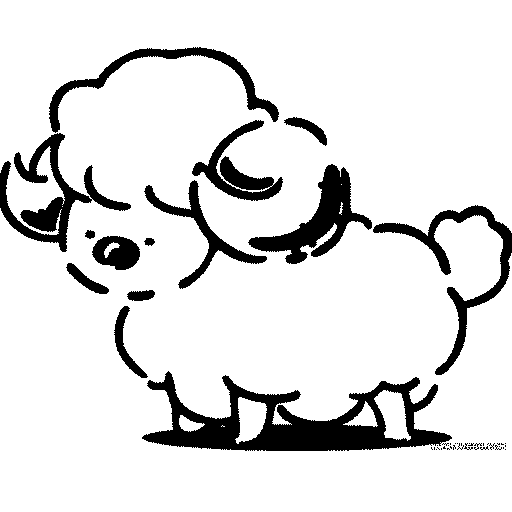
\includegraphics[width=2.3cm]{griffith-images/shengxiao/yang}
  
\includegraphics[width=2.3cm]{griffith-images/shengxiao/zhu}
  \caption{The ground-truth model parameters visualized as 12 512$\times$512 images.}
  \label{fig:ground-truth-shengxiao}
\end{figure}

\begin{figure}[!t]
  \centering
  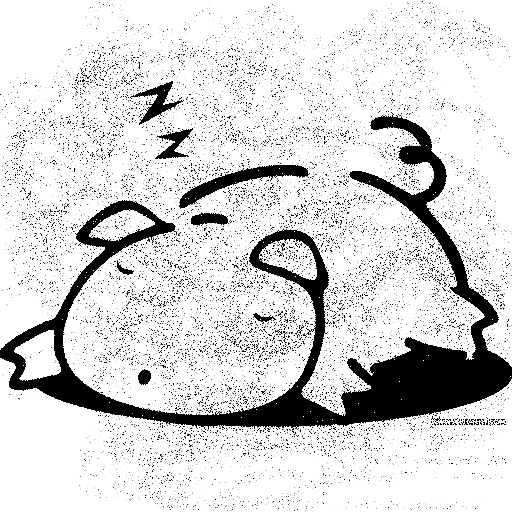
\includegraphics[width=2.3cm]{griffith-images/iteration-281/topic-00000}
  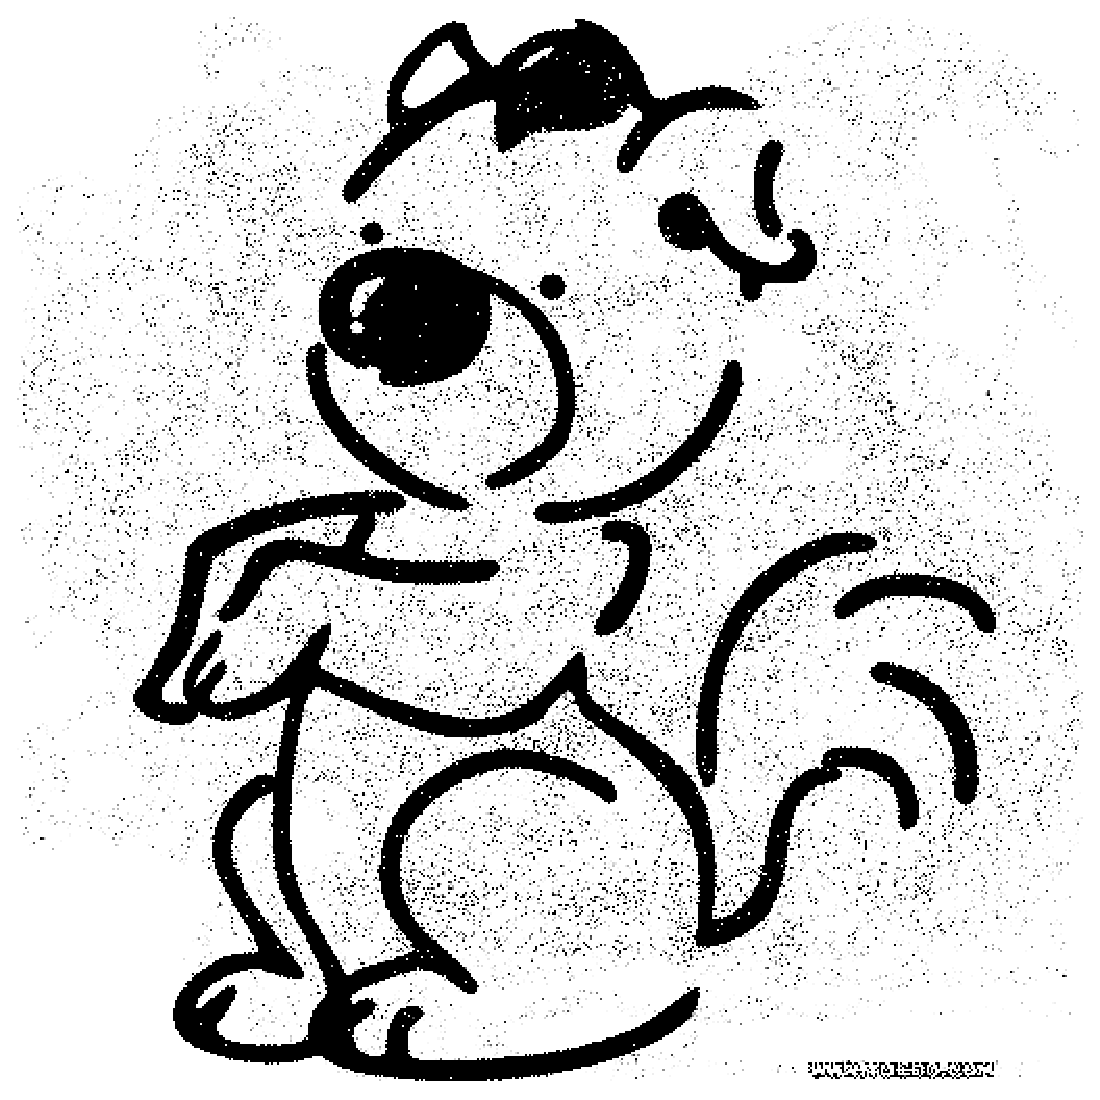
\includegraphics[width=2.3cm]{griffith-images/iteration-281/topic-00001}
  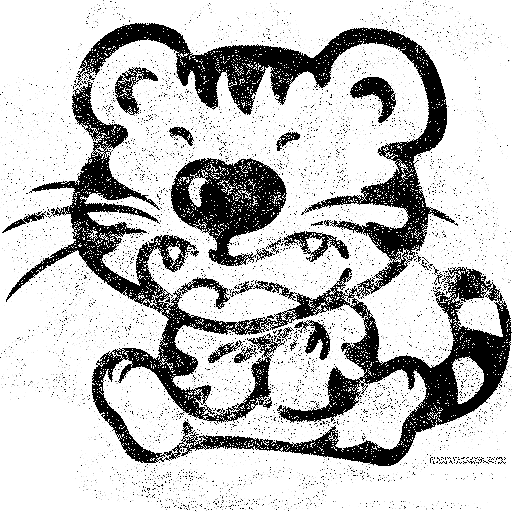
\includegraphics[width=2.3cm]{griffith-images/iteration-281/topic-00002}
  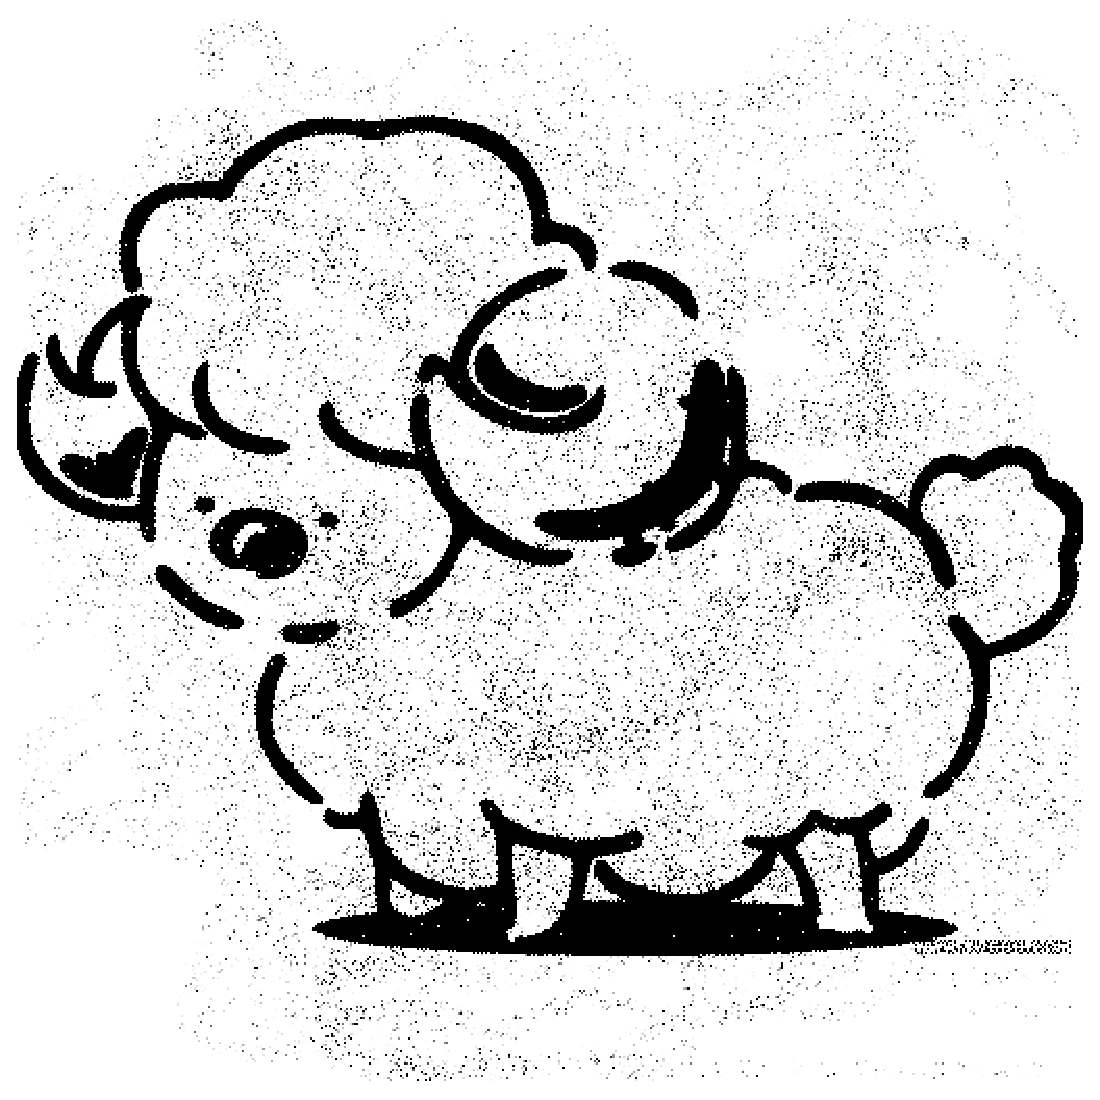
\includegraphics[width=2.3cm]{griffith-images/iteration-281/topic-00003}
  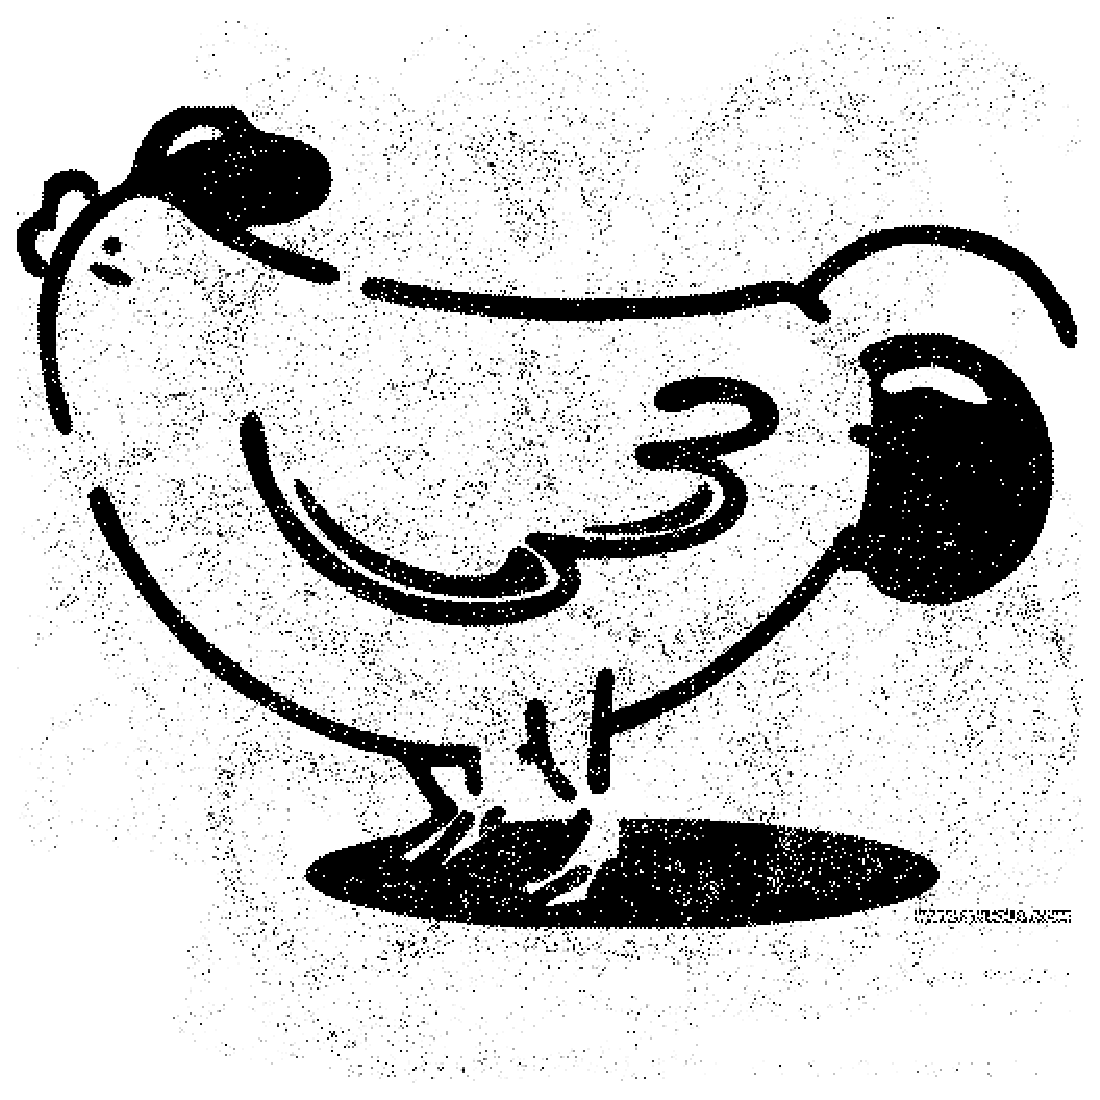
\includegraphics[width=2.3cm]{griffith-images/iteration-281/topic-00004}
  
\includegraphics[width=2.3cm]{griffith-images/iteration-281/topic-00005}
  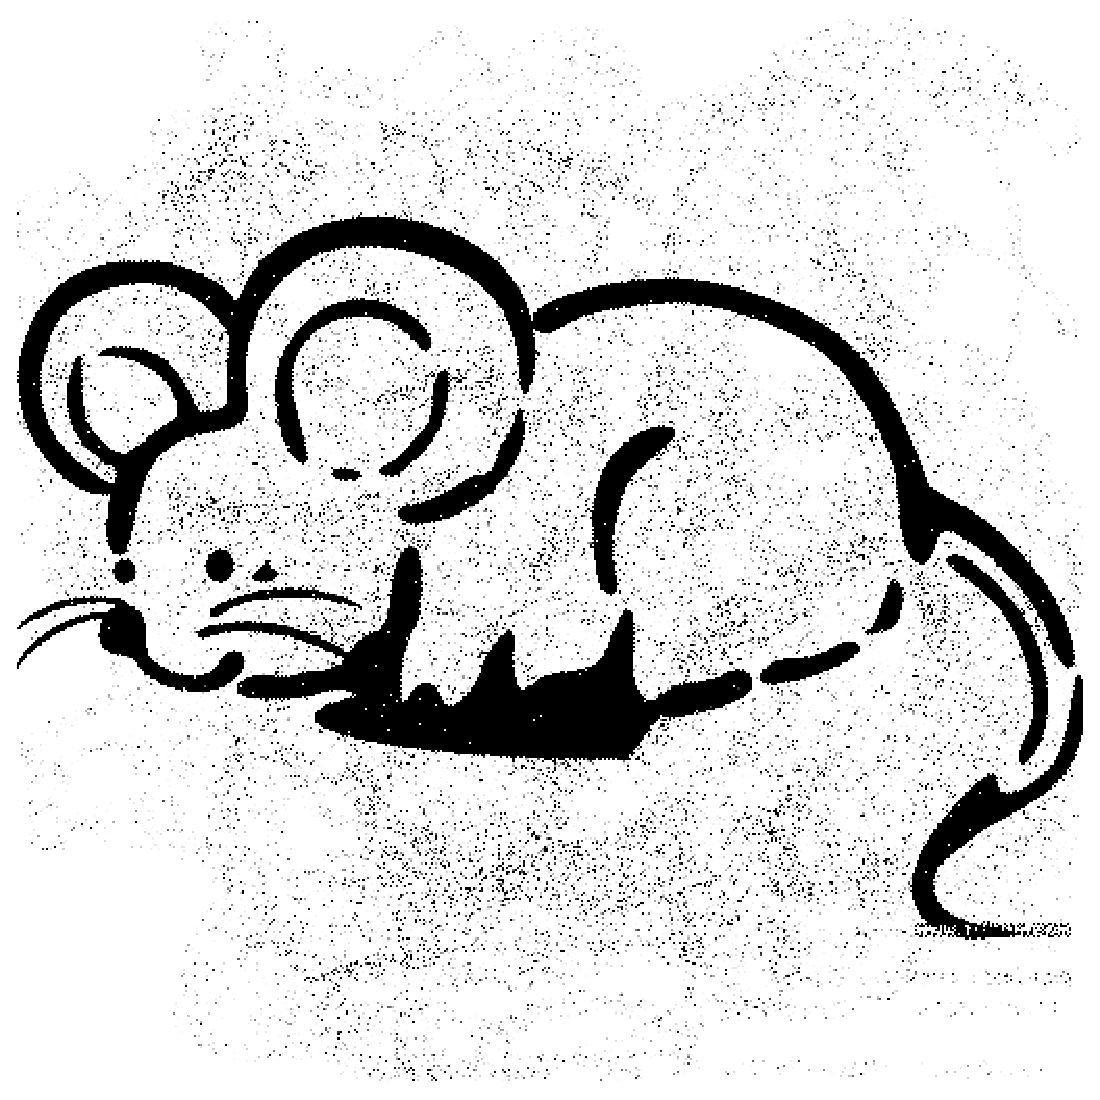
\includegraphics[width=2.3cm]{griffith-images/iteration-281/topic-00006}
  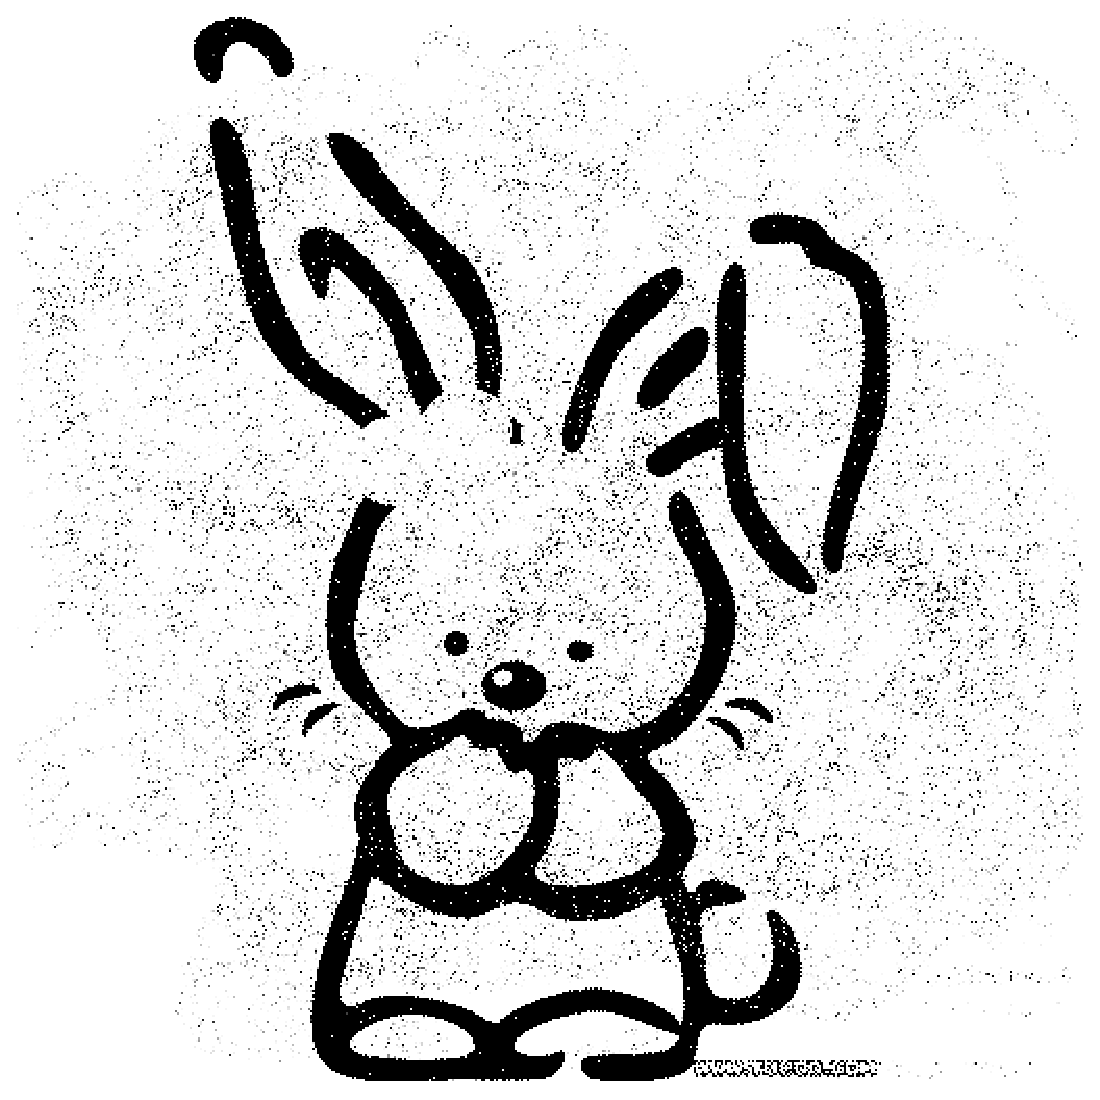
\includegraphics[width=2.3cm]{griffith-images/iteration-281/topic-00007}
  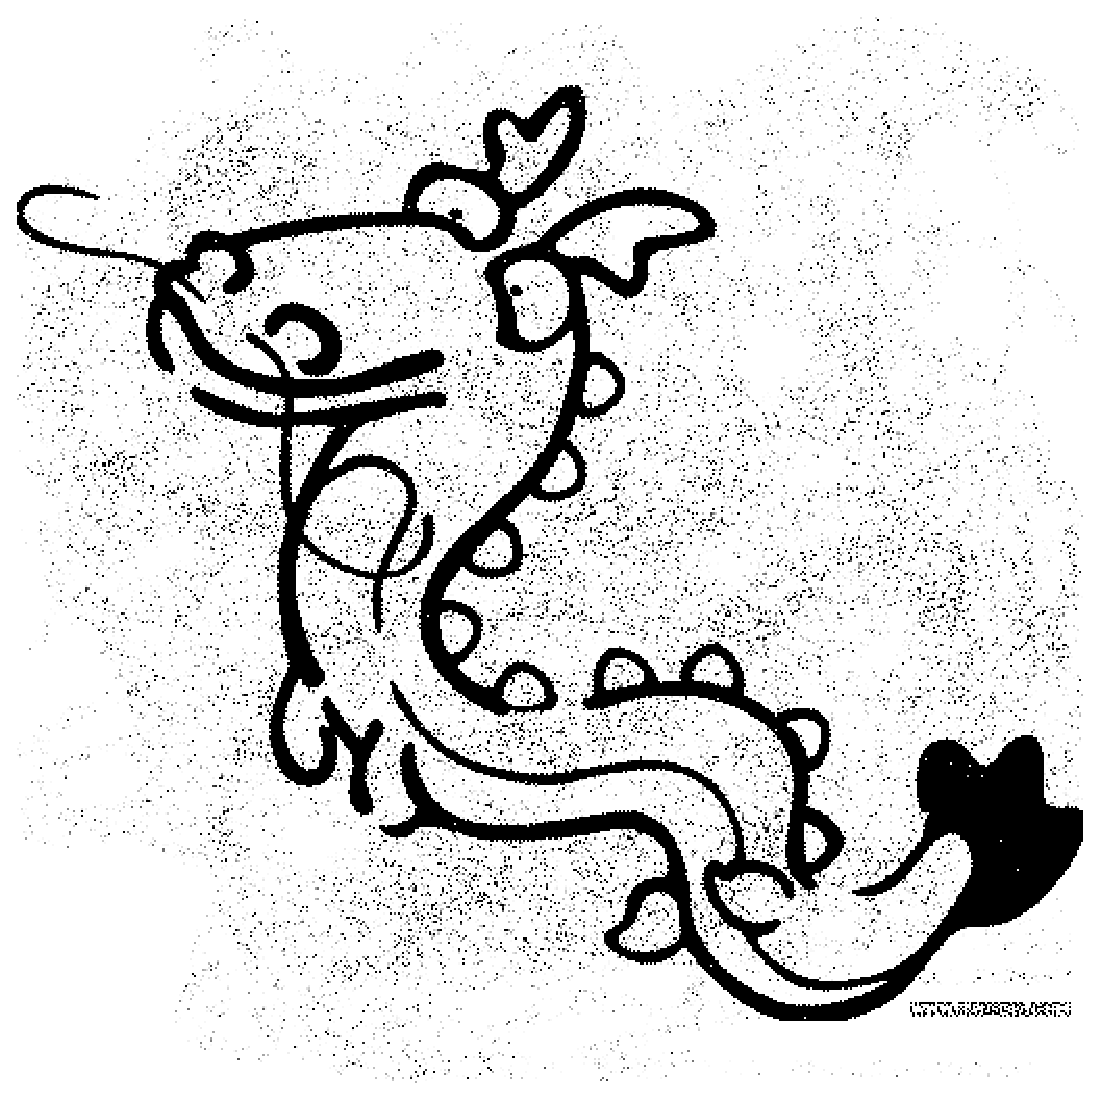
\includegraphics[width=2.3cm]{griffith-images/iteration-281/topic-00008}
  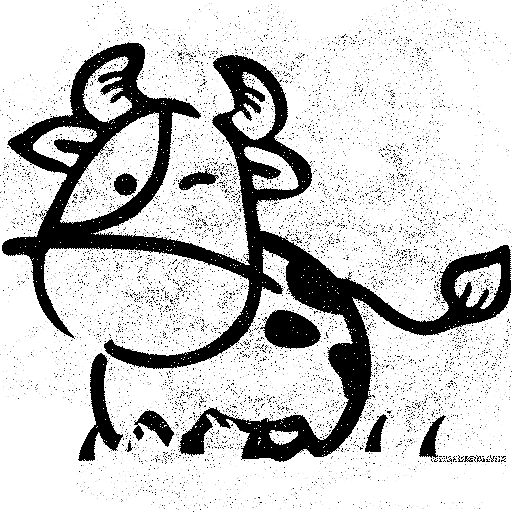
\includegraphics[width=2.3cm]{griffith-images/iteration-281/topic-00009}
  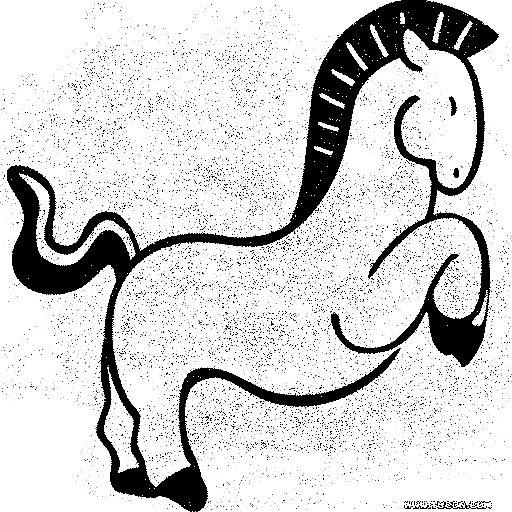
\includegraphics[width=2.3cm]{griffith-images/iteration-281/topic-00010}
  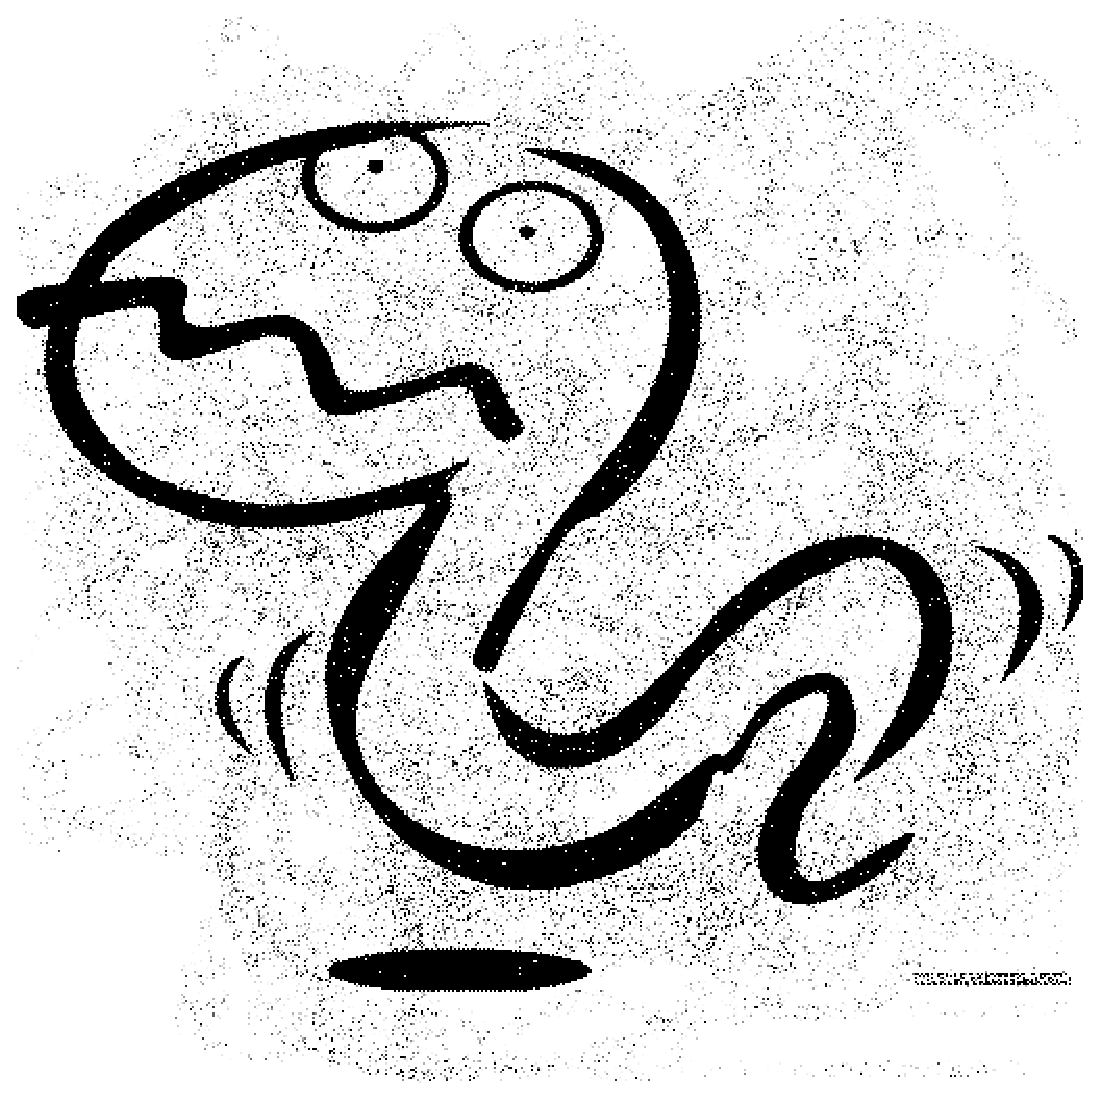
\includegraphics[width=2.3cm]{griffith-images/iteration-281/topic-00011}
  \caption{The model parameters estimated in the 281-th iteration.}
  \label{fig:learned-shengxiao}
\end{figure}

%%% Local Variables:
%%% mode: latex
%%% TeX-master: "llt"
%%% End:
